%%%%%%%%%%%%%%% Pacotes utilizados
\documentclass[a4paper, 12pt]{report}
\usepackage[T1]{fontenc}
\usepackage[brazil]{babel}
\usepackage[utf8]{inputenc}
\usepackage{verbatim}
\usepackage[normalem]{ulem} %para 
\usepackage{indentfirst}
\usepackage{setspace}
\usepackage{float}
\usepackage{fancyhdr}
\usepackage{titlesec}
\usepackage{capt-of}
\usepackage{setspace}
\usepackage{graphicx}
%%%%%%%%%%%%%%% Configurações
\setlength{\textwidth}{16cm}
\setlength{\textheight}{23cm}
\setlength{\evensidemargin}{-1cm} 
\setlength{\oddsidemargin}{0.5cm}
\setlength{\topmargin}{0cm}
\pagestyle{fancy}
\fancyhf{}
\lhead{\textbf{Nome:} Jhonatan Guilherme de Oliveira Cunha}
\rhead{\textbf{RA:} 2135590}
\cfoot{\thepage}
\hoffset= -0.4cm
\voffset=-0.9cm

\setstretch{1.5}

\titleformat{\chapter}{\normalfont\huge}{\textbf{\thechapter.}}{20pt}{\huge\bf}

\def\Cplusplus{C\raisebox{0.5ex}{\tiny\textbf{++}} }
%%%%%%%%%%%%% Início do documento
\begin{document}
	\hspace{2cm}

	\begin{large}
		\begin{center}
			\textbf{UNIVERSIDADE TECNOLÓGICA FEDERAL DO PARANÁ}\newline
			\textbf{CAMPUS CAMPO MOURÃO}
		\end{center}
	\end{large}
	
	\vspace{0.5cm}
	
	\begin{center}
		\textbf{RESENHA CAPÍTULO 2 E 9 - LIVRO ``Martin. Fowler. UML Essencial: Um Breve Guia para Linguagem Padrão. Martin Fowler; trad. João Tortello.– 3.ed. Porto Alegre: Bookman, 2005. ISBN: 8536304545.''}
	\end{center}

	\vspace{-1cm}
	{\let\clearpage\relax \chapter{Processo de Desenvolvimento}}
	
	Logo de inicio, o livro nos garante a ideia que, a maneira como utilizaremos a \textbf{UML} dependerá de qual processo utilizarmos. 
	
	O autor afirma que prefere utilizar o iterativo, porém, necessitando ser bem planejado para expor cedo os riscos e obter um melhor controle sobre o desenvolvimento. Sendo assim, apresentamos os processos mostrados no livro.
	
	\section{Processo Iterativo e Em Cascada}
	
	Quando estamos abordando estes dois tipos de processos, a principal diferença entre eles, é a maneira como subdividimos o projeto em segmentos menores.
	
	\subsection{Em Castata}
	Onde dividimos o projeto em atividades, por exemplo, nosso projeto poderia ter uma fase de dois meses de análise, seguida de um fase de projeto de quatro meses, três meses de codificação e três meses de testes, totalizando um ano inteiro construção de um software.
	
	Destacamos que, podem ocorrer necessidades de revisões das decisões de análise e projeto em etapas posteriores, porém, deve ocorrer o mínimo de vezes possível.

	\subsection{Iterativo}
	
	Neste dividimos o projeto em subconjuntos de funcionalidades, ou seja, dado 12 meses, subdividimos em 4 iterações. Sendo que em cada uma, concluímos o ciclo de vida do software referente a sua quantidade de requisitos ($1 \over 4$ de requisitos para cada itereção).
	
	Ao final de cada iteração, o ideal seria termos um software com qualidade de produção, porém, na maioria dos casos, necessitamos de um período para remover erros.
	
	Em momentos onde percebemos que não iremos conseguir finalizar todos os requisitos na iteração atual, utilizamos a técnica de \textbf{quadro de tempo}. Deslocando algumas funcionalidades para iterações posteriores.


	\section{Planejamento Preditivo e Adaptativo}
	
	Utilizamos o planejamento preditivo quando, realizamos o planejamento completo do software antes do processo começar, com objetivo de gerar maior entendimento posteriormente. Sendo dividido em duas etapas: a primeira sugere planos e é difícil prever, enquanto a segunda se torna mais previsível, pois os planos estão definidos.
	
	Um grande problema enfrentado pelo planejamento preditivo, é a revolução dos requisitos. Onde necessitamos realizar alterações, em etapas avançadas do projeto. Uma solução seria não permitir que as alterações sejam concluídas, porém, o software final pode não atender a demanda do cliente.

	Ao trabalharmos com o planejamento adaptativo, é obrigatório o uso do processo iterativo, pois precisaremos realizar algumas alterações durante a construção do \textit{software}.
	
	Desta forma, apresentamos duas recomendações extremamente válidas:
	
	\begin{enumerate}
		\item Não faça um plano preditivo até ter todos os requisitos precisos e exatos e até estar confiante de que eles não mudarão significativamente.
		
		\item Se não obter requisitos precisos e estáveis, utilize o planejamento adaptativo. 
	\end{enumerate}



	\section{Processos Ágeis}
	
	Os processos ágeis, primam que o sucesso de um projeto é devido a qualidade das pessoas que estão envolvidas nele e o quão bem trabalham juntas.
	
	As metodologias utilizam iterações curtas, frequentemente de um mês ou menos, desprezando o uso da \textbf{UML} no projeto. Os mesmos tendem a ter pouca formalidade, afirmando que o uso dela torna as alterações mais difíceis, indo contra a natureza das pessoas talentosas.
	
	
	\section{\textit{Rational Unified Process}}
	
	\textbf{RUP} trata-se de uma estrutura de processos, que fornece um vocabulário e uma vaga estrutura para falar sobre os processos. Em todos os casos de desenvolvimento, o \textbf{RUP} é um processo interativo. Todos os projetos \textbf{RUP} utiliza as quatro fases a seguir (temos algumas imprecisões sobre as fases):
	
	\begin{enumerate}
		\item A \textbf{concepção} faz uma analise inicial do projeto.
		
		\item A \textbf{elaboração} identifica os casos de usos principais do projeto e elabora o software em iterações, tendo no final uma boa ideia dos requisitos e um esqueleto funcional do sistema.
	
		\item A \textbf{construção} continua o processo, desenvolvendo funcionalidades suficientes para o lançamento.
		
		\item A \textbf{transição} inclui atividades que não realizamos no processo de forma iterativa.
	\end{enumerate}
	
	
	\section{Como adequar um processo a um projeto?}
	
	Não teremos um processo único que funcione para o desenvolvimento de todos os \textit{softwares}, sendo assim, em alguns casos necessitaremos adaptar processos.
	
	O livro aborda que, em desenvolvedores em experiências, é considerável utilizar um processo pronto, aprendendo como o mesmo funciona, para somente depois conseguir realizar alterações.
	
	Um bom método de adaptação dos processos, é realizar \textbf{retrospectivas de iteração}. Onde reunimos toda a equipe a fim de considerar falhas e como devem ser aprimoradas. Em reuniões mais curtas, podemos utilizar uma lista com três categorias.
	
	\begin{itemize}
		\item \textbf{Manter:} as coisas que funcionaram bem.
		\item \textbf{Problemas:} áreas que não estão funcionando bem.
		\item \textbf{Tentativa:} alterações para aprimorar o processo.
	\end{itemize}

	Durante nosso processo, utilizamos a UML para transmitir as ideias com mais clareza.

	
	\section{Análise de Requisito}
	
	Nesta etapa descobrimos o que o usuário e o cliente do software quer que ele faça, podemos violar algumas regras da \textbf{UML} para facilitar a comunicação com usuários e clientes, caso necessário. Veja abaixo algumas técnicas \textbf{UML} utilizadas durante este processo.
	
	\begin{itemize}
		\item Casos de uso, que descreve como as pessoas interagem com o sistema.
		
		\item Um diagrama de classe, sendo uma boa maneira para construir um vocabulário rigoroso do domínio.
		
		\item Um diagrama de atividades, mostrando o fluxo de como o software e as atividades humanas interagem.
		
		\item Um diagrama de estados, usado para mostrar as mudanças de estados que um objeto pode sofrer.
	\end{itemize}

	\section{Projeto}
	
	Quando estamos projetando um sistema, existe alguns diagramas \textbf{UML} mais técnicos que nos auxiliam bastante, sendo eles:
	
	\begin{itemize}
		\item \textbf{Diagrama de Classe} mostra as classes presentes no código e como elas se relacionam.
		
		\item \textbf{Diagrama de Sequência} para cenários mais comuns.
		
		\item \textbf{Diagrama de Pacote} mostra a organização em larga escala do software.
		
		\item \textbf{Diagrama de Estado} para classes com históricos de vidas complexos.
		
		\item \textbf{Diagrama de Distribuição} para mostrar o layout físico do software.
	\end{itemize}
	
	Muitas dessas técnicas podem ser utilizadas para documentar um software, quando já codificado. Esperamos também que, a implementação do código acompanhe o projeto \textbf{UML} feito, porém, em alguns casos necessitaremos realizar alterações em nossa modelagem.
		
		
	\section{Documentação}
	
	O autor do livro cita que, podemos utilizar diagramas \textbf{UML} para complementar a documentação de um software. Porém, precisamos construir uma documentação detalhada a partir do código de nosso sistema. Veja alguns exemplos de utilização de diagramas em documentações.
	
	\begin{itemize}
		\item \textbf{Diagrama de Pacotes:} ajuda a compreender as partes lógicas do sistemas, ver as dependências e mantê-las sobre controle.
		
		\item \textbf{Diagrama de Classe:} dentro do diagrama de pacote, o autor utiliza os diagramas de classe como um sumário gráfico.
		
		\item \textbf{Diagrama de Máquina de Estado:} caso nossas classes tenham um comportamento de ciclo de vida complexo, utilizamos este tipo de diagrama para descrevê-lo.
	\end{itemize}

	Devemos também documentar as medidas de projetos que não adotamos, e o motivo de não termos aplicado as mesmas.


	\section{Como entender um código legado?}
	
	Podemos utilizar diagramas para conseguir entender um emaranhado de código, uma boa estrategia é utilizar diagramas de sequência para ver como vários objetos colaboram no tratamento de um método complexo.
	
	
	{\let\clearpage\relax \chapter{Casos de Uso}}
	
	Os casos de uso fornecem uma narrativa de como nosso software é utilizado, ou seja, descreve as interações típicas entre os usuários do sistema.
	
	Segundo o autor, é mais fácil descrever os casos de uso utilizando cenários. Um cenário é uma sequência de passos que descreve uma interação entre um usuário e um sistema (descrevendo todos os casos possíveis).
	
	\section{Conteúdo de um caso de uso}
	
	Cada caso de uso possui um ator principal (usuário) que pede para o sistema executar um serviço. Podem existir outros atores que nosso sistema se comunica enquanto executa o caso de uso, eles são chamados de atores secundários.
	
	Em cada passo de nosso caso de uso, devemos declarar de forma simples, mostrando claramente quem está executando determinado passo (cada passo demonstra a intenção do ator).
	
	Uma extensão dentro do caso de uso mostra diferentes cenários que nosso software pode tomar, para isso, devemos nos perguntar em cada passo: ``Como isso poderia ser feito de uma outra forma? O que poderia dar errado?''. Veja na Figura \ref{CasoDeUsoProduto} um exemplo onde temos um texto de caso de uso e suas respectivas extensões.
	
	
	\begin{figure}[H]
		\centering
		\includegraphics[scale=0.5]{casoDeUso.png}
		\label{CasoDeUsoProduto}
		\caption{Exemplo texto de caso de uso.}
	\end{figure}


	Podemos ter um caso de uso incluído em outro, ou seja, um passo complicado de um caso de uso, pode ser um outro caso de uso. Esta subdivisão é útil em situações onde, um passo complexo congestionaria nosso sistema principal, ou em passos repetidos em vários casos de uso. Desta forma, podemos adicionar algumas informações importantes em cada caso de uso.
	
	\begin{itemize}
		\item \textbf{Pré-Condição:} informa o que o sistema deve garantir como verdadeiro antes de começar o caso de uso.
		
		\item \textbf{Garantia:} descreve o que o sistema deve assegurar no fim de cada caso. As garantias de sucesso se mantem em cenários bem-sucedidos, e as mínimas após qualquer cenário.
		
		\item \textbf{Gatilho:} especifica o evento que inicia o caso de uso.
	\end{itemize}

	Lembre-se de sempre tentar manter cada caso de uso breve e fácil de ler.
	
	
	\section{Diagramas de Casos de Uso}
	
	A \textbf{UML} não nos diz nada sobre o conteúdo de um caso de uso, porém, nos fornece um formato de diagrama para mostrá-lo. Veja na Figura \ref{diagramaCasoDeUso} um exemplo de diagrama de caso de uso.
	
	\begin{figure}[H]
		\centering
		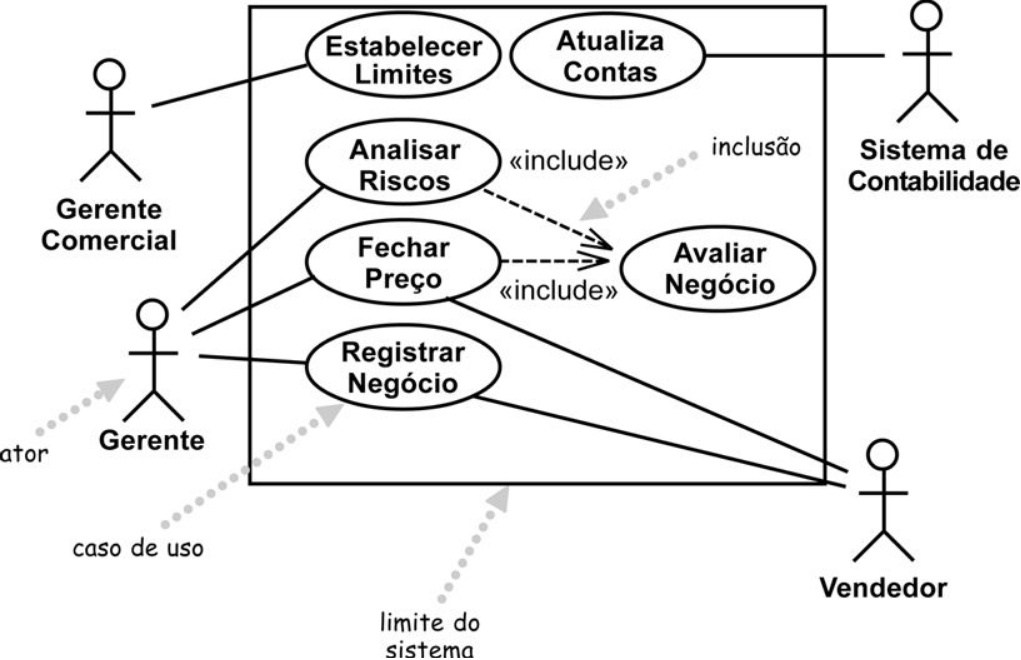
\includegraphics[scale=0.5]{diagrama.png}
		\label{diagramaCasoDeUso}
		\caption{Diagrama caso de uso.}
	\end{figure}
	
	O diagrama acima serve como ferramenta de sumário gráfico, ou seja, conseguimos mostrar os atores, os casos de uso e os relacionamento entre eles.
	
	\section{Caso de Uso e Funcionalidades}
	
	As funcionalidades constituem uma boa maneira de repartir	 um sistema para planejarmos de maneira iterativa. Enquanto os casos de uso servem para descrever em forma narrativa como os atores (usuários) utilizam o sistema.
	
	
	\section{Quando utilizar casos de uso?}
	
	Primeiramente, devemos deixar claro que, o caso de uso representa um visão externa do sistema, não tendo nenhuma correlação com as classes do mesmo.
	
	Desta forma, devemos montar nossos casos de usos com fácil legibilidade, intencionado a ajudar o entendimento dos requisitos funcionais do sistema. Algumas versões detalhados poderão ser feitas antes do desenvolvimento desse caso de uso.
	
	Concentraremos nossas energias no modo texto do caso de uso, pois o mesmo contém todo valor da técnica necessária.
	
	
\end{document}
